\documentclass[english,10pt,aspectratio=169]{beamer}

\usepackage{amsmath}
\usepackage[T1]{fontenc}
\usepackage{listings}
\usepackage{tikz}
\usepackage{ulem}

\mode<presentation>
\usetheme{Singapore}
\usecolortheme{orchid}

\lstdefinestyle{PythonStyle}{
	basicstyle=\scriptsize\ttfamily,
	language=Python,
	numbers=left,
	tabsize=4
}
\lstset{basicstyle=\small,style=PythonStyle}

\def\presentationtitle{\textbf{
	Spending less time bug fixing by \\
	spending more time unit testing
}}

\title{\large\presentationtitle}
\author{\textbf{
	<Name>
}}
\date{}

\begin{document}

\begin{frame}
	\titlepage
\end{frame}

\begin{frame}
	\begin{quote}
		There's much more to unit testing than the act of writing tests.
		\begin{flushright}
			\tiny{---Khorikov, \textup{Unit Testing Principles, Practices, and Patterns}, 3}
		\end{flushright}
	\end{quote}
\end{frame}

\begin{frame}{The goal of unit testing}
	To enable \textbf{sustainable} growth of software project.
	\begin{columns}[T]
		\begin{column}{0.5\textwidth}
			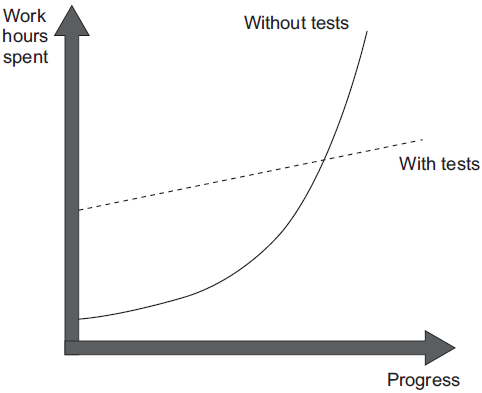
\includegraphics[width=\textwidth]{images/vs_no_test.png}
		\end{column}
		\begin{column}{0.5\textwidth}
		\end{column}
	\end{columns}
\end{frame}

\begin{frame}{The goal of unit testing}
	To enable \textbf{sustainable} growth of software project.
	\begin{columns}[T]
		\begin{column}{0.5\textwidth}
			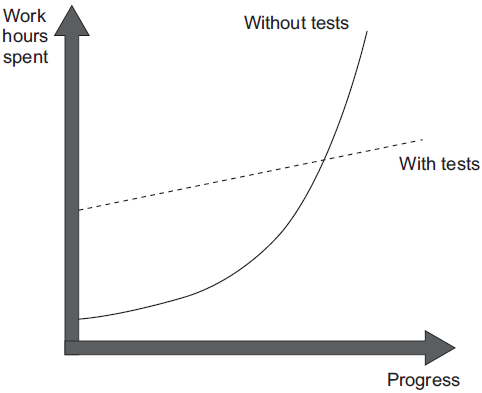
\includegraphics[width=\textwidth]{images/vs_no_test.png}
		\end{column}
		\begin{column}{0.5\textwidth}
			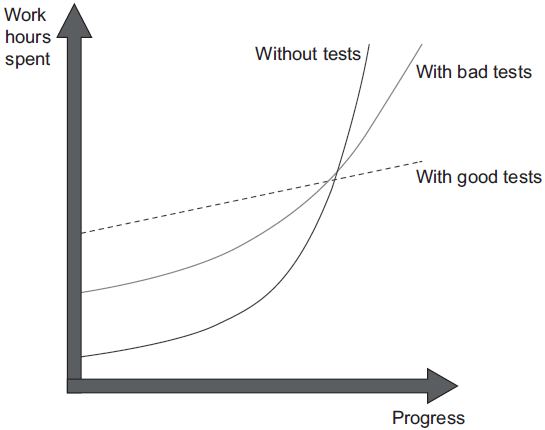
\includegraphics[width=\textwidth]{images/vs_bad_test.png}
		\end{column}
	\end{columns}
\end{frame}

\defverbatim[colored]\coveragecode{%
\begin{lstlisting}[linewidth=0.5\textwidth]
def is_fizzbuzz(num: int) -> bool:
	if num % 3 and num % 5:
		return True
	return some_var

def test_fizzbuzz():
	result = is_fizzbuzz(3)
	assert result
\end{lstlisting}
}
\begin{frame}{Coverage metrics}
	Statement vs Branch vs \sout{Path} vs \sout{Condition}
	\begin{columns}[T]
		\begin{column}[]{0.5\textwidth}
			\begin{minipage}{\linewidth}
				\coveragecode
			\end{minipage}
		\end{column}
		\begin{column}[]{0.5\textwidth}
			\begin{flalign*}
 				&\frac{Number\ of\ statements\ executed}{Total\ number\ of\ statements}\\
				\approx\ &67 \%
			\end{flalign*}
		\end{column}
	\end{columns}
\end{frame}

\defverbatim[colored]\coveragecodetwo{%
\begin{lstlisting}[linewidth=0.5\textwidth]
def is_fizzbuzz(num: int) -> bool:
	return True if num % 3 and num % 5 else some_var

def test_fizzbuzz():
	result = is_fizzbuzz(3)
	assert result
\end{lstlisting}
}
\begin{frame}{Coverage metrics}
	Statement vs Branch vs \sout{Path} vs \sout{Condition}
	\begin{columns}[T]
		\begin{column}[]{0.5\textwidth}
			\begin{minipage}{\linewidth}
				\coveragecodetwo
			\end{minipage}
		\end{column}
		\begin{column}[]{0.5\textwidth}
			\begin{flalign*}
 				&\frac{Number\ of\ statements\ executed}{Total\ number\ of\ statements}\\
				=\ &100 \%
			\end{flalign*}
		\end{column}
	\end{columns}
\end{frame}
\end{document}
